\subsection{Стохастическая чувствительность}

    Для аппроксимации вероятностного распределения случайных состояний вокруг детерминированных аттракторов (равновесия, циклов или хаоса) можно использовать метод функции стохастический чувствительности. Данный подход описан в работе Ряшко Л. Б. \cite{Ryashko}.

    Стохастическая чувствительность равновесия \(\bar{x}\) вычисляется по формуле:

    \[
        M = \frac{s(\bar{x})}{1 - q(\bar{x})},
    \]

    где 

    \[
        q(x) = \left[\frac{\partial f}{\partial x}(x, 0)\right]^2 \quad s(x) = \left[\frac{\partial f}{\partial \eta}(x, 0)\right]^2.
    \]

    Стохастическая чувствительность \(k\)-циклов можно вычислить по формулам:

    \[
        M_{t + 1} = q_t M_t + s_t \quad q_t = q(\bar{x_t}) \quad s_t = s(\bar{x_t}),
    \]

    \[
        M_1 = \frac{r_{k + 1}}{1 - q_1 \cdot \ldots \cdot q_k}.
    \]

    То есть набор элементов \(\{M_1, \cdots, M_k\}\) определяет значения стохастической чувствительности \(k\)-цикла. Для вычисления требуется знать \(r_{t + 1}\), который можно найти по формуле \(r_{t + 1} = q_t r_t + s_t\), \(t \in \overline{1, k}\) и \(r_1 = 0\).

    Стохастическая чувствительность хаоса вычисляется по формулам:

    \[
        M(c_1) = \left[\frac{\partial f}{\partial x}(f(c_{-1}, 0), 0)\right]^2 s(c_{-1}) + s(f(c_{-1}, 0)) \quad M(c) = s(c_{-1}),
    \]

    где \(c_{-1}\) --- прообраз критической точки, \(c = f(c_{-1}), c_1 = f(c)\).

    Полоса рассеивания строится по формулам: 

    \begin{equation}
        \label{scattering_band}
        x_\varepsilon = x^* \pm 3\varepsilon \sqrt{M},    
    \end{equation}

    где \(x^*\) --- одно из значений аттрактора при фиксированном \(\beta\). Формула для вычисления значения \(M\) выбирается в зависимости от вида аттрактора, для которого строится полоса рассеивания.

    На рисунках \ref{SSF_max} и \ref{SSF_min} изображены максимум и минимум значений функции стохастической чувствительности соответственно. Красные линии соответствуют модели с \(\alpha\)-шумом, синии линии --- модели с \(\beta\)-шумом, а зеленые --- модели с аддитивным шумом.

    \begin{figure}
        \centering
        \subfloat[Минимум]{
            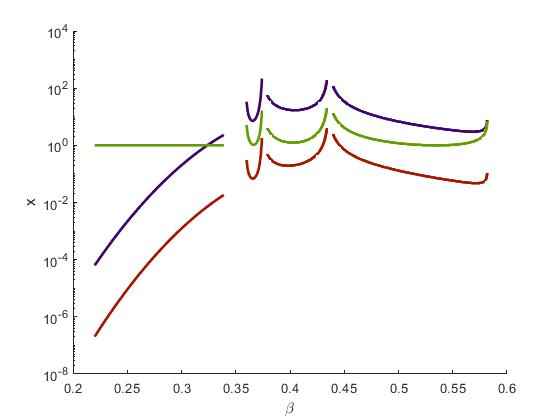
\includegraphics[width=0.5\textwidth]{stochastic/images/SSF_min.jpg}
            \label{SSF_min}
        }
        \subfloat[Максимум]{
            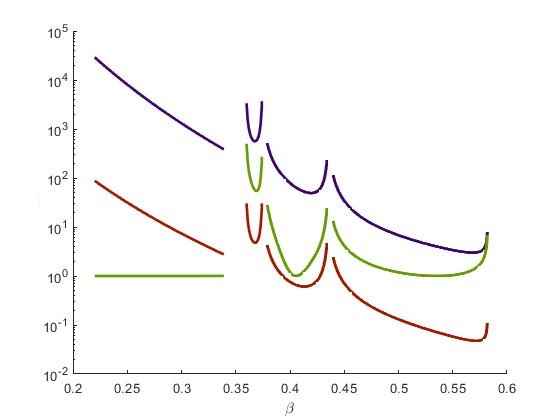
\includegraphics[width=0.5\textwidth]{stochastic/images/SSF_max.jpg}
            \label{SSF_max}
        }  
            
        \captionsetup{justification=centering}
        \caption{Функции стохастической чувствительности для моделей (\ref{alpha_chaos}), (\ref{beta_chaos}) и (\ref{additive_chaos}) (красный, синий и зеленый соответственно)}
    \end{figure}
  
    На рисунке \ref{bifurcation_x_0_2_a_1_beta_chaos_fss} красными линиями изображена полоса рассеивания вокруг стохастических состояний системы (\ref{beta_chaos}) с \(\beta\)-шумом при интенсивности \(\varepsilon = 0.001\). 

    \begin{figure}
        \centering
        \subfloat[Общий вид стохастической диаграммы и доверительной полосы]{
            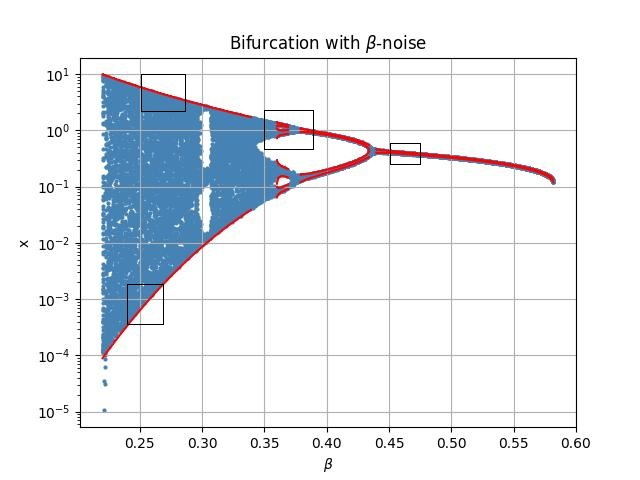
\includegraphics[width=0.7\textwidth]{stochastic/images/bifurcation_x_0_2_a_1_beta_noise_fss.jpg}
            \label{bifurcation_x_0_2_a_1_beta_chaos_fss}
        }

        \subfloat[полоса для равновесия]{
            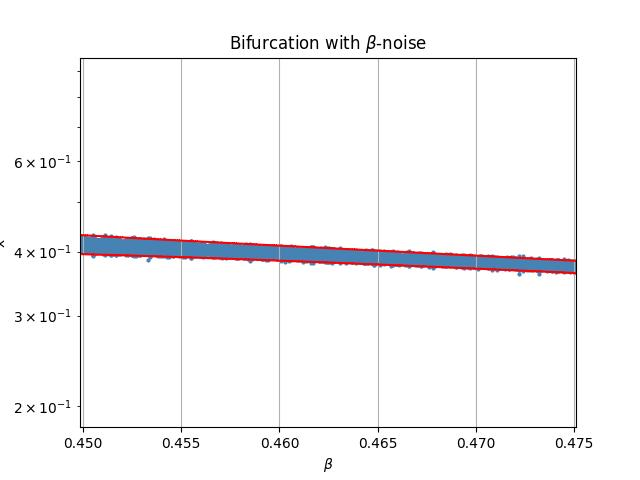
\includegraphics[width=0.5\textwidth]{stochastic/images/bifurcation_x_0_2_a_1_beta_noise_fss_segment_stable.jpg}
            \label{bifurcation_x_0_2_a_1_beta_chaos_fss_segment_stable}
        }  
        \subfloat[полоса для 4-цикла]{
            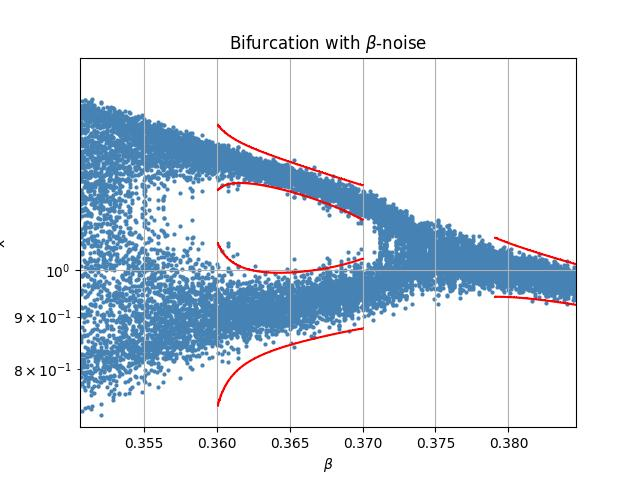
\includegraphics[width=0.5\textwidth]{stochastic/images/bifurcation_x_0_2_a_1_beta_noise_fss_segment_2_cycle.jpg}
            \label{bifurcation_x_0_2_a_1_beta_chaos_fss_segment_2_cycle}
        }
            
        \subfloat[полоса для хаоса]{
            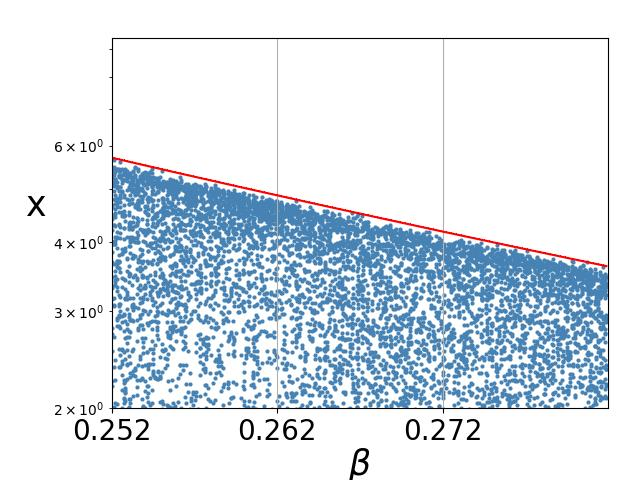
\includegraphics[width=0.5\textwidth]{stochastic/images/bifurcation_x_0_2_a_1_beta_noise_fss_segment_chaos_up.jpg}
            \label{bifurcation_x_0_2_a_1_beta_chaos_fss_segment_chaos_up}
        }
        \subfloat[полоса для хаоса]{
            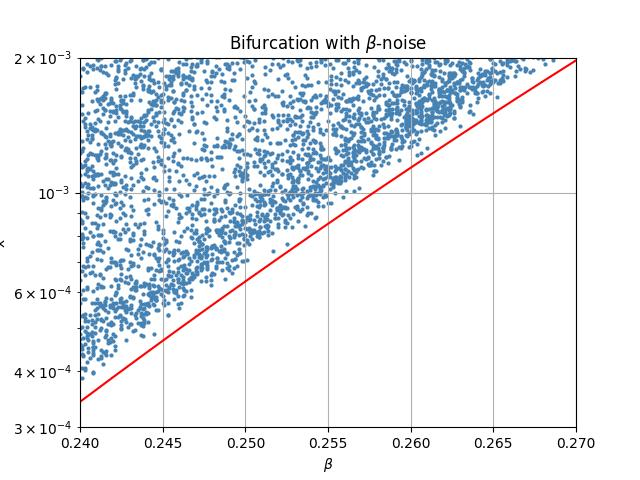
\includegraphics[width=0.5\textwidth]{stochastic/images/bifurcation_x_0_2_a_1_beta_noise_fss_segment_chaos_down.jpg}
            \label{bifurcation_x_0_2_a_1_beta_chaos_fss_segment_chaos_down}
        }
            
        \captionsetup{justification=centering}
        \caption{Доверительная полоса для модели \ref{beta_chaos} (с \(\beta\)-шумом) при \(\varepsilon = 0.001\)}
    \end{figure}

    Увеличенный участок от \(\beta \approx 0.45\) до \(\beta \approx 0.48\) изображен на рисунке \ref{bifurcation_x_0_2_a_1_beta_chaos_fss_segment_stable}. Видно, что случайные состояния почти всегда находятся внутри полосы рассеивания, построенной по правилу трех сигм. 

    На участках с k-циклами и хаосом (рисунки \ref{bifurcation_x_0_2_a_1_beta_chaos_fss_segment_2_cycle}, \ref{bifurcation_x_0_2_a_1_beta_chaos_fss_segment_chaos_up} и \ref{bifurcation_x_0_2_a_1_beta_chaos_fss_segment_chaos_down}) будет наблюдаться аналогичная ситуация: значения лежат внутри полосы рассеивания.

    Таким образом, наблюдается хорошее согласование эмпирических данных и теоретической аппроксимации их разброса.